%%%%%%%%%%%%%%%%%%%%%%%%%%%%%%%%%%%%%%%%%%%%%%%%%%%%%%%%%%%%%%%%%%%%%%%%%%%%%%%%

\documentclass[letterpaper, 10 pt, conference]{ieeeconf}  
                                                          
%\documentclass[a4paper, 10pt, conference]{ieeeconf}      
                                                          
\overrideIEEEmargins

% The following packages can be found on http:\\www.ctan.org
%\usepackage{graphics} % for pdf, bitmapped graphics files
%\usepackage{epsfig} % for postscript graphics files
\usepackage{mathptmx} % assumes new font selection scheme installed
%\usepackage{times} % assumes new font selection scheme installed
\usepackage{amsmath} % assumes amsmath package installed
\usepackage{amssymb}  % assumes amsmath package installed
\usepackage{float}
\usepackage{array}
\usepackage[spanish]{babel}
\usepackage{comment}
\usepackage{graphicx}


\title{\LARGE \bf
SDMT Alternative Analysis
}

\author{Pedro Vladimir Hern\'andez Serrano}
\begin{document}

\maketitle
\thispagestyle{empty}
\pagestyle{empty}


%%%%%%%%%%%%%%%%%%%%%%%%%%%%%%%%%%%%%%%%%%%%%%%%%%%%%%%%%%%%%%%%%%%%%%%%%%%%%%%%
\begin{abstract}

It was replicated the stages of reliability and validity

\end{abstract}

%%%%%%%%%%%%%%%%%%%%%%%%%%%%%%%%%%%%%%%%%%%%%%%%%%%%%%%%%%%%%%%%%%%%%%%%%%%%%%%%
\section{Introduction}
\vspace{2mm}
The SDMT has proven to be quite useful in neuropsychological MS research. It has excellent test–retest reliability, and alternate forms have been developed that are equivalent in difficulty. When the alternate forms are used, reliability is maintained. Validity research shows that SDMT is a good measure of processing speed or efficiency. SDMT is the neuropsychological test most sensitive to MS cognitive disorder and correlates very well with MRI measures of atrophy, lesion burden, and micro- structural pathology. The test very effectively repre- sents the core neuropsychological domain of processing speed.
In comparison to other digit/symbol substitution tests, the digital version has the following advantages: limited practice effect due to the generation of new keys and forms at each session, standardisation of the presentation, precision in the presentation of the stimulus and scoring of the responses, and immediate classification of each subject score according to normative values

The main difference of responding the SDMT test on paper and responding on digital is thet the second one we have the precise moment every patient performs a task, so we might discover new features as time.
We are interested on analyse the time of response every participant have, in addition, we want to check the practicing effect on trials over the time

%%%%%%%%%%%%%%%%%%%%%%%%%%%%%%%%%%%%%%%%%%%%%%%%%%%%%%%%%%%%%%%%%%%%%%%%%%%%%%%%
\section{Methods}
\vspace{2mm}

\subsection{Study}
We choose the score variable as the number of correct answers on every test

Study performed from 2017-05-31 to 2017-08-10

We expect that every person performs the test within 8 or 10 times, we found  9.479.47  on average.
The number of days of the study on every participant should be 30 days, we found  (9.47∗3.33=31.55)(9.47∗3.33=31.55)  The expected number of trials times the expected days between every trial we can find an inference for the days.

Patients on MS group: 15 (65.0\%)
Patients on HC group: 8 (35.0\%) 

Group	Average Time of Response
MS	3.82 Seconds
HC	3.35 Seconds

Order	1	2	3	4	5	6	7	8	9
MS	Mult	Star	Plus	Triangle	Inf	Square	Hamburger	Window	Circle
HC	Plus	Star	Mult	Triangle	Inf	Square	Hamburger	Window	Circle

Average Number of Event per Group 
 MS Group: 11.93 (SD 4.59) 
 HC Group: 8.38 (SD 3.11)

Computing Intervals for every group 

Average Score of MS Group: 46.22 (SD 7.88) 
SEM (Standard Error): 2.03 
True Score Interval:[42.2359279085235, 50.211286981849291]

Average Score of HC Group: 52.92 (SD 8.22)
SEM (Standard Error): 2.91 
True Score Interval:[47.223154935582976, 58.613704038776]

As we can see both distributions looks pretty Gaussian, so we might perform a test to prove that all the scores of MS patients have a normal distribution, the same with HC participants

Mean MS: 46.22 Interval: [42.2359279085235, 50.211286981849291]
Mean HC: 52.92 Interval: [47.223154935582976, 58.613704038776]
At this point it does not seems to be any difference in standard deviation on both groups, is clear to see an important difference between the 2 groups on average score

\begin{figure}[ht]
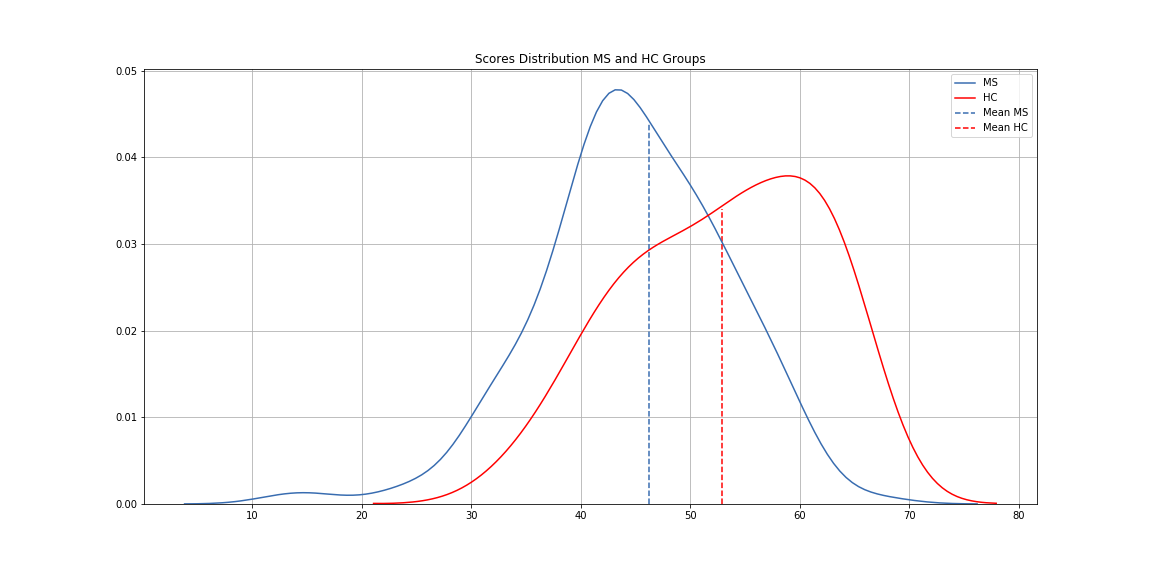
\includegraphics[width=9cm]{scores_distribution_grid.png}
\caption{Scores Distribution}
\label{tab:scores}
\end{figure}

\vspace{2mm}

\subsection{Statistics}

\input{summary1}


\section{Results}
\vspace{2mm}

\subsection{Test-Restest Reliability}

Average Days Between Test-retest: 14.7 (SD): 3.21

Test-Retest Reliability:
 MS: 0.84   p-value: 8.496653745316737e-05
 HC: 0.85   p-value: 0.006935033738858537

\begin{figure}[ht]
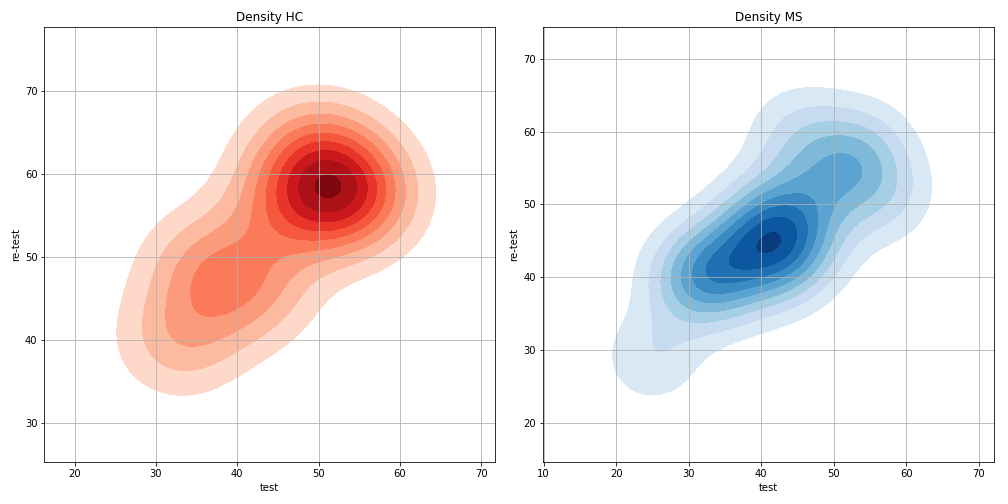
\includegraphics[width=8cm]{test-retest_density_grid.png}
\caption{Test Re-test Density}
\label{tab:density}
\end{figure}

Is it possible to see the correlation between test and retest on both groups, also is intuitive to see that people is scorimng more on the second one, showing an effect of improving

Standar Error of Measurement: 
 MS: 2.274577217805805
 HC: 2.004522634546915
 
 The MDC, representing the magnitude of change necessary to exceed the measurement the error of two repeated measures at a specified CI was calculated for the 95% CI as:
 $$MDC_{95} = SEM( 1.96 )(\sqrt{2})$$
 

 Minimal Detectable Change: 
 MS: 6.304806382168228 
 HC: 5.556253267885786
It means that if a measure is more than that so it's an outlier


Effect Size

Cohen`s d-value: 0.837
Benedict 2016	 d=1.11d=1.11 	Large (Cohen, 1988)
Orikami 2017	 d=0.837d=0.837 	Large (Cohen, 1988)

MS Morning: 45.7 (SD 7.61)
MS Afternoon: 43.92 (SD 9.33)
HC Morning: 52.36 (SD 8.82)
HC Afternoon: 53.53 (SD 8.68)
There's not significance difference between means, so it means that a person is going to score alike no matter the moment on the day. But in the other hand is clearly to see that respond in the morning for MS group is presumably less variance

Difference in Variance for MS: 66.52%  p-value: 0.0285

Difference in Variance for HC: 97.0%  p-value: 0.466

There's an statistical significant difference between the variance between morning and afternoon on MS group, it means that people perform more constant over the time if they respond in the morning, in the other hand, it shows also a big difference for HC, but we got a big p-value, so we cannot reject the null hypothesis for HC group


Practicing Effect
3.1 Effect on Median Time of Response
We should find if there is statistical difference on the first median time a person performed and the last median time the person performed, we use the d-Cohen value to find an effect split on MS and HC groups

Cohens d-value, First Median vs Last Median: 
 MS: 0.754 Large 
 HC: 0.974 Large


Average Score of MS Group: 
 First: 4186.53 (SD 803.87) 
 Last: 4186.53 (SD 803.87) 
Cohens d-value: 0.415   Ttest pvalue=0.0802

Average Score of HC Group: 
 First: 3798.62 (SD 631.04) 
 Last: 3798.62 (SD 631.04) 
Cohens d-value: 1.037   Ttest pvalue=0.000176

\input{top10_fcc}

In order to prove validity, we need to be able to predict who is an MS person
Predictive validity
This is the degree to which a test accurately predicts a criterion that will occur in the future. For example, a prediction may be made on the basis of a new intelligence test, that high scorers at age 12 will be more likely to obtain university degrees several years later. If the prediction is born out then the test has predictive validity.

Source	Accuracy	Specificity	Sensitivity
Akbar 2011	0.78	0.84	0.71
Ruet 2013	0.77	0.85	0.60
Van Schependom 2014	NA	0.60	0.91
Orikami
Inference	0.67	0.69	0.66
k-NN	0.79	0.80	0.79
Naive Bayes	0.79	0.80	0.79
Logistic	0.84	0.85	0.84

\begin{figure}[ht]
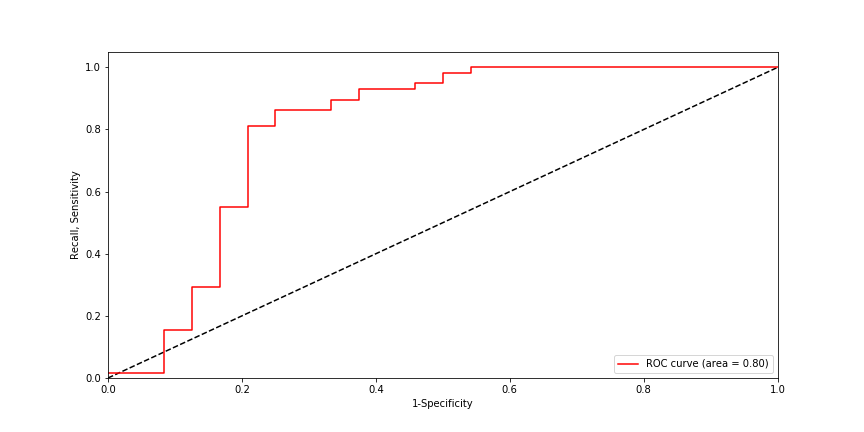
\includegraphics[width=9cm]{roc_logistic.png}
\caption{ROC Logistic}
\label{tab:roc}
\end{figure}


\section{Discussion}

On the study the recomendations it's been followed in order to accomplish the correct Reliability of the expermiment and after watch the results we might say that the test is Reliable there's only the consideration on the number of participants to perform the study

In the literature there's more than one method to measure the difference between the statistic of two populations, on this study it is been used the d-Cohen's value and the F test for difference in variance

We reject the null hypothesis on MS group, so it means that there is 68\% greater the variance of scores if the patients respond in the morning, rather than the afternoon.
In the other hand we can not reject the null hypothesis on the HC group because there's no much data points, that means that we might not say anything about how late the participant in HC perform the test

In the literature shows that exist practicing effect and more significant after longer testing period
Not influenced by gender, age, relapses, disability progression and prior natalizumab treatment
They conclude that the practicing effect is less if they are more impaired on the EDSS scale
\vspace{3mm}

Distraction Points as a MS Feature

It is mainly important to analyze all the features involved in every test taken by a person, and it is straightforward thinking that not all tasks are with full concentration because the nature of the tool, is an app, and we might expect the people taking the test can get distracted by some random reason
The main objective here is to analyze any pattern related to the time in milliseconds a participant spend on responding every visual task.

Standart Deviation of every delta per group 
 MS: 663.6751885085198 
 HC: 502.5068924690813
 
  One person, one event¶
We can just take one single event on a random choise person (eobt3CosDzEtxWW5P) for instance, and plot the time of response in milisecond alongside the 90 seconds showing the symbols choosen on each task

As we might see the points outside of the boundaries are distraction points because they are 2 SD of the median time of response, where the SD corresponds the variance of the group.

Group	Average Score	Average Distractions
MS	52.91	1.81
HC	46.22	1.49

As we may see on the plots above we see a negative and significative correlation, the MS group is more clear. The more distractions the less score
The number of distractions that a single person has is a clear feature that helps to classify the MS people, this feature does not deoend in demographic variables but just with in the test behaviour
\begin{figure}[ht]
\includegraphics[width=9cm]{distraction_sample.png}
\caption{Distraction Points}
\label{tab:dis}
\end{figure}

he general performance is acceptable, and at some point better than the references, tryying more type of validity is going to make clear the complete validity of the test
The next steps should be try concurrent validity correlating scores on MS people with impairment data, job information or fMRI results





%%%%%%%%%%%%%%%%%%%%%%%%%%%%%%%%%%%%%%%%%%%%%%%%%%%%%%%%%%%%%%%%%%%%%%%%%%%%%%%%


%%%%%%%%%%%%%%%%%%%%%%%%%%%%%%%%%%%%%%%%%%%%%%%%%%%%%%%%%%%%%%%%%%%%%%%%%%%%%%%%




\begin{thebibliography}{10}

\bibitem{c1} Daron Acemoglu and Asu Ozdaglar, Graph Theory and Social Networks, Lecture 2, MIT, September 14, 2009.
\bibitem{c2} John Adrian Bondy, Graph Theory with Applications.	Mathermathics: Amsterdam, 1976.
\bibitem{c3} Sonal Raj, Neo4j High Performance.	Packt Publishing, March 2015.
\end{thebibliography}




\end{document}
